\documentclass[hidelinks,12pt,a4paper,oneside]{article}

\usepackage{setspace}
\usepackage[utf8]{inputenc}
\usepackage[russian]{babel}
\usepackage{fancyhdr}
\usepackage{graphicx}
\usepackage{tabularx}
\usepackage{lipsum}
\usepackage{enumitem}
\usepackage{graphicx}
\usepackage{minipage-marginpar}
\usepackage[absolute,overlay]{textpos}
  \setlength{\TPHorizModule}{1mm}
  \setlength{\TPVertModule}{1mm}
\usepackage{xcolor}
\usepackage{hyperref}
\hypersetup{
    colorlinks=true,  
    urlcolor=blue
}

\usepackage[a4paper,left=3cm,right=2cm,top=2.5cm,bottom=2.5cm]{geometry}
 \geometry{
 a4paper,
 total={170mm,257mm},
 left=10mm,
 top=5mm,
bottom = 6mm
 }
\onehalfspacing

\begin{document}
%
%
% ENGLISH VERSION OF RESUME
%
%
\thispagestyle{empty}
{ \LARGE Anton Gromov }
\noindent{\rule{12cm}{0.5mm}}
{\large
\begin{itemize}[topsep=5pt, itemsep=-11pt]
	\item[] Novosibirsk, Russia
	\item[] Phone : 8-962-840-62-50
	\item[] E-mail : \href{mailto://gromoff97@mail.ru}{gromoff97@mail.ru}
	\item[] Skype : gromoff97
	\item[] Github : \href{https://github.com/gromoff97}{github.com/gromoff97}
	\item[] Birthdate : Aug 22, 1997
\end{itemize}
}
   \begin{textblock}{20}(130,12)
      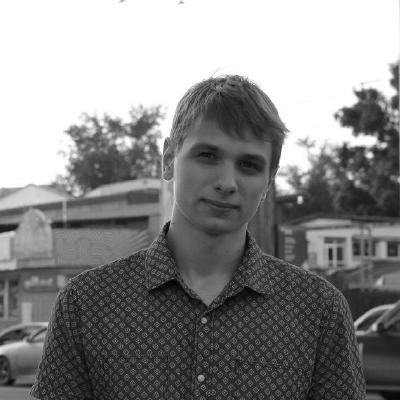
\includegraphics[scale=0.33]{myphoto.jpg}
    \end{textblock}

%\noindent{\rule{17cm}{0.5mm}}
\ 
\\[2px]
{\Large \underline{\textbf{Goal}}} :\\[4px]
{\large Position of "Java"\ developer with possibilty of professional growth.} \\[3px]
{\Large \underline{\textbf{Summary}}} : 
{\large
\begin{itemize}[noitemsep]
	\item JVM languages ( Core 'Java' /  'Groovy' );
	\item 1.5 - year experience in unit testing with 'JUnit', 'TestNG' and 'Spock'- frameworks.
	\item 1-year experience in using 'Selenium'-framework;
	\item Understanding of SQL – queries (DDL, DML, DCL, Тransactions. most used DBMS -  'PostgreSQL');
	\item 4 years experience in using 'UNIX'--like OSs ('FreeBSD', 'Arch Linux', 'Kali Linux');
	\item Experience in Shell-scripting and system programming in 'UNIX'-- like OSs;
	\item Experience in using VCSs ( 'Git' , 'Subversion' );
	\item Experience with imperative and declarative build tools ( Apache 'Maven' , 'Make'-utility , Apache 'Ant' )
	\item Writing and speaking English skills at Upper-Intermediate level (B2/2).
\end{itemize}
 }
\ \\
{\Large \underline{\textbf{Experience}}} : \\ [6px]
{\large
“Sberbank”,\ Saint-Petersburg {\small( since 01.2020 to present )} \\
Senior Test Automation Engineer ("EKS"\ and "PPRB": UI/API test-automation)
}\par\noindent\rule{\textwidth}{0.4pt}
{\large
“Performance Lab”,\ Novosibirsk {\small( 06.2019 - 12.2019 )} \\
Software Test Automation Engineer ("EKS": internal API test - automation)
}\par\noindent\rule{\textwidth}{0.4pt}
{\large
“Performance Lab”,\ Saint-Petersburg {\small( 12.2018 - 06.2019 )} \\
Software Test Automation Engineer ("UXCrowd": UI test - automation) 
}\par\noindent\rule{\textwidth}{0.4pt}
{\large
“Define Developers”,\ Saint-Petersburg {\small( 03.2018 - 12.2018 )} \\
Junior "PHP"\ - \ developer (Basic REST-services improvings and "bugfixing") \\
}
\ \\
{\Large \underline{\textbf{Education}}} : \\ [8px]
{\large
ITMO University\ , Saint-Petersburg \\
Faculty of Software Engineering and Computer Systems
}
\newpage
\thispagestyle{empty}
{ \LARGE Антон Громов }
\noindent{\rule{12cm}{0.5mm}}
{\large
\begin{itemize}[topsep=5pt, itemsep=-11pt]
	\item[] Россия, Новосибирск
	\item[] Телефон : 8-962-840-62-50
	\item[] E-mail : \href{mailto://gromoff97@mail.ru}{gromoff97@mail.ru}
	\item[] Skype : gromoff97
	\item[] Github : \href{https://github.com/gromoff97}{github.com/gromoff97}
	\item[] Дата рождения : 22.08.1997
\end{itemize}
}
   \begin{textblock}{20}(125,11)
      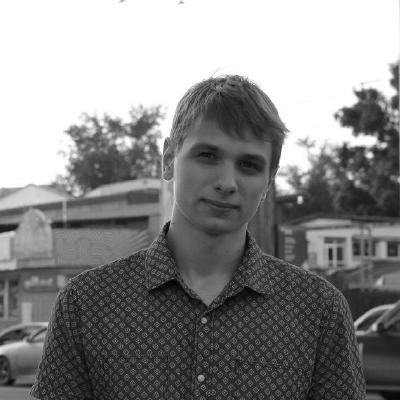
\includegraphics[scale=0.33]{myphoto.jpg}
    \end{textblock}

\ 
\\[1px]
{\Large \underline{\textbf{Цель}}} :\\[4px]
{\large Позиция 'Java'-разработчика с возможностью профессионального роста.} \\[3px]
{\Large \underline{\textbf{Коротко о навыках}}} : 
{\large
\begin{itemize}[noitemsep]
	\item JVM - языки ( Core 'Java' /  'Groovy' );
	\item 1,5 года опыта в использовании таких unit-testing фреймворков, как  'JUnit', 'TestNG' и 'Spock'.
	\item Год опыта использования фреймворка 'Selenium';
	\item Понимание SQL – запросов (DDL, DML, DCL, Транзакции. чаще всего используемая СУБД -  'PostgreSQL');
	\item 4 года опыта эксплуатации 'UNIX'--like операционных систем ('FreeBSD', 'Arch Linux', 'Kali Linux');
	\item Опыт Shell-скриптинга и системного программирования в 'UNIX'-- like операционных системах;
	\item Опыт работы с системами контроля версия ( 'Git' , 'Subversion' );
	\item Опыт работы с императивными и декларативными системами сборки ( Apache 'Maven' , 'Make'-utility , Apache 'Ant' )
	\item Уровень владения английским языком на уровне "Upper-Intermediate" (B2/2).
\end{itemize}/
 }
\vspace{-20px}
\ \\
{\Large \underline{\textbf{Опыт}}} : \\ [6px]
{\large
ПАО “Сбербанк”,\ Санкт-Петербург {\small( с 01.2020 по настоящее время )} \\
Старший инженер по разработке ("ЕКС" и "ППРБ" : API/UI test - automation)
\vspace{-10px}
}\par\noindent\rule{\textwidth}{0.4pt}
{\large
“Performance Lab”,\ Новосибирск {\small( 06.2019 - 12.2019 )} \\
Инженер по автоматизации тестирования ("ЕКС" : internal API test - automation)
\vspace{-25px}
}\par\noindent\rule{\textwidth}{0.4pt}
{\large
“Performance Lab”,\ Санкт-Петербург {\small( 12.2018 - 06.2019 )} \\
Инженер по автоматизации тестирования ("UXCrowd" : UI test-automation)
\vspace{-10px}
}\par\noindent\rule{\textwidth}{0.4pt}
{\large
“Define Developers”,\ Санкт-Петербург {\small( 03.2018 - 12.2018 )} \\
Junior "PHP"\ - \ разработчик  (Basic REST-services improvings and "bugfixing") \\
}
\ \\
{\Large \underline{\textbf{Образование}}} : \\ [8px]
{\large
Университет "ИТМО"\ , г. Санкт-Петербург \\
Факультет программной инженерии и компьютерной техники.
}
\end{document}